\chapter{Architecture de communication}


	\section{Définition d'une architecture de communication}
Quand on parle d'Architecture, on se réfère à une structure d'éléments définissant un système complexe. Dans le langage courant, l'architecture est ``l'art de concevoir et de construire un bâtiment selon des règles techniques'' (Le Petit Larousse). Pour un informaticien, il est fait souvent référence à l'architecture du calculateur, ensemble structuré d'éléments électroniques et logiques.

L'Architecture de Communication définit l'ensemble des entités nécessaires à la Communication ainsi que les règles régissant les échanges entre elles. On parle aussi d'Architecture de Réseau.

Pour bien comprendre les notions sous-jacentes à l'architecture de communication, prenons un exemple d'une communication entre individus par l'intermédiaire du réseau postal:

Le responsable d'une entreprise française (FR) négocie un marché avec le responsable d'une entreprise brésilienne (BR). Pour cela, un échange de documents en langue anglaise (langue commune) entre les deux responsables est réalisé. Le processus d'échange peut-être décrit de la façon suivante (on supposera que pour chaque fonction bien identifiée, un service est requis):
\begin{enumerate}
\item FR rédige le document explicitant les conditions du marché; FR confie ce document au service de traduction pour effectuer la traduction et se charger de l'envoi;
\item Le traducteur effectue la traduction et confie le document au service secrétariat pour envoi;
\item Le secrétaire référence le document et demande au service courrier de s'occuper de l'envoi;
\item Le service courrier en fonction de la qualité de service requise pour cet envoi choisit le mode d'acheminement (courrier postal, fax, messager,\ldots)  le plus approprié, précise l'adresse complète du destinataire final et expédie le document;
\item L'acheminement se fera à travers différents réseaux des différents pays en utilisant l'adresse du site destination ainsi que les informations de trafic;
\item Sur chaque liaison traversée, des mécanismes de contrôle sont mises en oeuvre pour s'assurer de la non altération du document transporté;
\item Selon le service support utilisé, une interface spécifique et une représentation physique de l'information est mise en oeuvre;
\end{enumerate}

Des fonctions similaires seront mises en oeuvre du coté destinataire en remontant les différentes couches.

\section{Les services offerts par une architecture de communication}
Les services offerts par une architecture de communication couvrnt tous les aspects de la transmission physique jusqu'à la synchronisation des processus applicatifs :
\begin{description}
	\item[Transmission physique] Correspond au supports, au type d'encodage, aux liaisons, toute l'architecture physique.
	\item[Contrôle d'erreurs]  Vérifier que les paquets sont bien arrivés.
	\item[Contrôle de flux]  S'assurer que l'émetteur n'aille pas trop vite par rapport au récepteur
	\item[Routage]  en cas de nœud de communication, choisir le chemin le plus rapide ceci en fonction du trafic. 
	\item[Régulation de flux (congestion)] Réguler le flux pour éviter la congestion\footnote{Peut être assimiler aux bouchons}, il préfère la prévention afin d'éviter les bouchons. 
	\item[Séquencement]  Les fichiers sont découpés en plusieurs paquets, en effet un paquet à une taille maximum, le séquencement réassemble les paquets afin de reconstituer le fichier grâce à une numérotation des paquets..
	\item[Contrôle de bout en bout] Vérifier que le fichier à bien été reconstitué. 
	\item[Gestion du dialogue] 
	\item[Reprise sur incidents]Cela permet aussi de gérer un arrêt de la connexion réseau afin de reprendre le transfert à l'endroit où il s'était arrêté
	\item[Transformation de l'information] Codage de l'information (avec le code ASCII par exemple), compression (codecs), sécurité de l'information (cryptage) 
	\item[Synchronisation des processus] Sémantique de l'application, c'est-à-dire quelle opération au niveau applicatifs (Renommer un fichier, créer un répertoire, \ldots)
\end{description}

\section{Pourquoi normaliser l'architecture ?}
Les opérateurs de Télécommunications, réunis au sein du CCITT (ITU actuellement), ont défini des architectures de communications permettant l'échange d'informations. Ainsi, leurs réseaux étaient interopérables ce qui a permis la constitution de réseaux internationaux.

Le monde Informatique n'a pas réagi de la même façon. Les intérêts n'étaient pas les mêmes. Au début de l'ère informatique, les constructeurs ont défini des Architectures de Communication permettant l'échange de données entre leurs équipements informatiques. Ainsi, IBM a défini SNA (Systems Network Architecture), DEC a défini DNA (Digital Network Architecture)\ldots Ces Architectures avaient l'inconvénient majeur d'être trop souvent liées à des équipements spécifiques : ce sont des Architectures Constructeurs ou des Architectures Propriétaires. L'aberration de cette situation se répercuta sur les utilisateurs : par exemple une agence de voyages devait se munir d'autant de terminaux que de Systèmes Informatiques différents auxquels elle devait accéder. Des îlots de réseaux de constructeurs s'étaient formés.

Face à cette situation, en 1977, l'organisation ISO a constitué des comités pour le développement d'une architecture commune permettant la connexion des équipements et l'échange de données entre eux. Ainsi, au sein du Comité Technique (TC : Technical Committee) TC97, deux Sous Comités (SC : SubCommittee) SC6 et SC21 s'occupèrent de la normalisation dans le domaine des Télécommunications et de l'Interconnexion de Systèmes. Le premier modèle a été achevé en 1979. En 1984, ISO publia le document ISO 7498 relatif au modèle de référence pour l'Interconnexion de Systèmes Ouverts OSI (Open Systems Interconnection). Le modèle OSI est référencé au CCITT sous la norme X.200. 

	Des \textbf{architectures normalisées} ont été mis en place par les opérateurs de Télécommunications (X21, X25, ISDN,\ldots).\\
	Des \textbf{architectures propriétaires} ont également être mise en place par les constructeurs informatiques (SNA, DNA, DSA).\\
	\begin{description}
		\item[1977] \textbf{ISO} constitue un comité pour la normalisation dans le domaine des télécommunications et de l'interconnexion des systèmes.\\
		\item[1984] ISO 7948 référence CCITT X.200 (ITU)
		\item[OSI] Cadre fonctionnel -- Le modèle de référence. Les objectifs du modèle OSI sont les suivants : 
			\begin{itemize}
				\item Décomposer (décomposition fonctionnelle)
				\item Structurer
				\item Assurer l'indépendance vis à vis du matériel et du logiciel.
			\end{itemize}
	\end{description}
\section{Le modèle OSI}
\subsection{Utilité et objectifs}
On appelle Système Ouvert Réel un système réel dont la communication avec un autre système réel se fait conformément au modèle OSI.

Le modèle OSI définit un cadre fonctionnel pour l'élaboration de normes d'interconnexion de systèmes. En aucun cas, OSI ne décrit comment ces systèmes fonctionnent en interne ou comment les normes doivent être implantées. OSI est un modèle et non une pile de protocoles.

Les objectifs du modèle OSI sont :
\begin{itemize}
	\item Décomposer et structurer le système de communication en éléments directement réalisables (Décomposition fonctionnelle) ;
	\item Assurer le maximum d'indépendance vis à vis du matériel et du logiciel ;
\end{itemize}

SI regroupe les entités en 7 couches. Chaque couche correspond à un niveau logique de fonctions. On distingue :
\begin{itemize}
	\item Les couches basses (1-4) relatives au transfert de l'information ;
	\item Les couches hautes (5-7) relatives au traitement réparti de l'information ;
\end{itemize}

\newpage
\subsection{Les couches}
\begin{verbatim}
      +-------------------+ Exemple  
7 N+4 |   Application     | HTTP   
      +-------------------+     
6 N+3 |   Présentation    | HTML, MPEG     
      +-------------------+              SERVICES APPLICATIFS (Couches hautes)
5 N+2 |   Session         |   
      +-------------------+ ===========================================================
4 N+1 |   Transport       | TCP 
      +-------------------+    
3 N   |   Réseau          | IP    
      +-------------------+                 SERVICES TRANSPORTS(Couches basses)
2 N-1 |   Liaison         | Wifi    
      +-------------------+    
1 N-2 |   Physique        | RJ45  
      +-------------------+  
\end{verbatim}
\subsubsection{Couche 1}
1. Couche Physique : Elle s'occupe de la transmission des bits de façon brute sur un canal de communication. Cette couche doit garantir la parfaite transmission des données (un bit 1 envoyé doit bien être reçu comme bit valant 1). Concrètement, cette couche doit normaliser les caractéristiques électriques (un bit 1 doit être représenté par une tension de 5 V, par exemple), les caractéristiques mécaniques (forme des connecteurs, de la topologie\ldots), les caractéristiques fonctionnelles des circuits de données et les procédures d'établissement, de maintien et de libération du circuit de données. ;
\subsubsection{Couche 2}
2. Couche Liaison de Données : Son rôle est un rôle de ``liant'' : elle va transformer la couche physique en une liaison a priori exempte d'erreurs de transmission pour la couche réseau. Elle fractionne les données d'entrée de l'émetteur en trames, transmet ces trames en séquence et gère les trames d'acquittement renvoyées par le récepteur. La couche liaison de données doit être capable de renvoyer une trame lorsqu'il y a eu un problème sur la ligne de transmission. De manière générale, un rôle important de cette couche est la détection et la correction d'erreurs intervenues sur la couche physique. Cette couche intègre également une fonction de contrôle de flux pour éviter l'engorgement du récepteur.
\subsubsection{Couche 3}
3. Couche Réseau : C'est la couche qui permet de gérer le sous-réseau, i.e. le routage des paquets sur ce sous-réseau et l'interconnexion des différents sous-réseaux entre eux. Au moment de sa conception, il faut bien déterminer le mécanisme de routage et de calcul des tables de routage (tables statiques ou dynamiques\ldots). La couche réseau contrôle également l'engorgement du sous-réseau. On peut également y intégrer des fonctions de comptabilité pour la facturation au volume, mais cela peut être délicat.
L'unité d'information de la couche réseau est le paquet.
\subsubsection{Couche 4}
4. Couche Transport : Si la couche réseau rend le service de transfert d'informations de terminal réseau à terminal réseau, la couche transport contrôle le transfert de bout en bout (d'utilisateur final à utilisateur final). Le rôle principal de la couche transport est de prendre les messages de la couche session, de les découper s'il le faut en unités plus petites et de les passer à la couche réseau, tout en s'assurant que les morceaux arrivent correctement de l'autre côté. Cette couche effectue donc aussi le réassemblage du message à la réception des morceaux.Cette couche est également responsable du type de service à fournir à la couche session, et finalement aux utilisateurs du réseau : service en mode connecté ou non, avec ou sans garantie d'ordre de délivrance, diffusion du message à plusieurs destinataires à la fois\ldots Cette couche est donc également responsable de l'établissement et du relâchement des connexions sur le réseau. Un des tous derniers rôles à évoquer est le contrôle de flux.
\subsubsection{Couche 5}
5. Couche Session : La session de transfert d'informations peut subir divers incidents. Un service de reprise sur incidents peut être nécessaire. D'autre part, des outils nécessaires à la gestion du dialogue peuvent être utilisés. Cette couche organise et synchronise les échanges entre tâches distantes.
\subsubsection{Couche 6}
6. Couche Présentation : Il ne suffit pas de transférer les données. Il faut aussi les interpréter en vue d'une bonne coopération. La syntaxe des données échangées entre entités applicatives est définie à ce niveau. Typiquement, cette couche peut convertir les données, les reformater, les crypter et les compresser.
\subsubsection{Couche 7}
7. Couche Application : Elle comprend les programmes d'applications ainsi que des fonctions applicatives génériques permettant le développement d'applications distribuées.

\subsection{Intéraction entre entités}
Nous utilisons la notation '(N)' pour signifier `` de rang N''.

La technique de structuration de base du Modèle OSI est la structure en couches : chaque système est logiquement composé d'un ensemble ordonné de sous-systèmes représentés verticalement. Voilà quelques définitions.
\subsubsection{Définitions}
\begin{description}
	\item[Sous-système (N)]\'Elément de rang N d'une division hiérarchique d'un système n'ayant d'interactions qu'avec les éléments des niveaux immédiatement supérieur et inférieur de cette division.
	\item[Couche (N)] Subdivision de l'architecture OSI, constituée de sous-systèmes de rang N. On dit qu'une couche fournit un service ou qu'elle est prestataire de services.
	\item[Entité (N)] Élément actif d'un sous-système (N).
	\item[Service] Capacité que possède la couche (N) -et les couches inférieures à celle-ci, fournie aux entités (N+1), à la frontière entre la couche (N) et la couche (N+1). Ces services sont invoqués par des primitives, spécifiques du service.
	\item[Facilité (N)]Élément d'un service (N).
	\item[Point d'accès à des services\footnote{Service Acces point ou SAP}] Point où les services (N) sont fournis par une entité (N) à une entité (N+1).
	\item[Protocole (N)] Ensemble de règles et de formats (sémantiques et syntaxiques) déterminant les caractéristiques de communication des entités (N) lorsqu'elle effectuent les fonctions (N).
\end{description}

Chaque couche (N) fournit des services (N) aux entités (N+1) de la couche (N+1). Les services d'une couche (N) sont fournis à la couche (N+1) grâce aux fonctions effectuées à l'intérieur de la couche (N) et, au besoin, avec l'aide des services offerts par la couche (N-1).
La coopération entre entités (N) est régie par un ou plusieurs protocoles (N).

\begin{figure}[H]
	\centering
	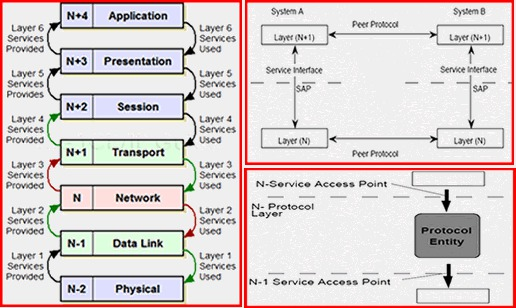
\includegraphics[width=15cm]{partie1/interaction.jpg}
\end{figure}
\begin{figure}[H]
	\centering
	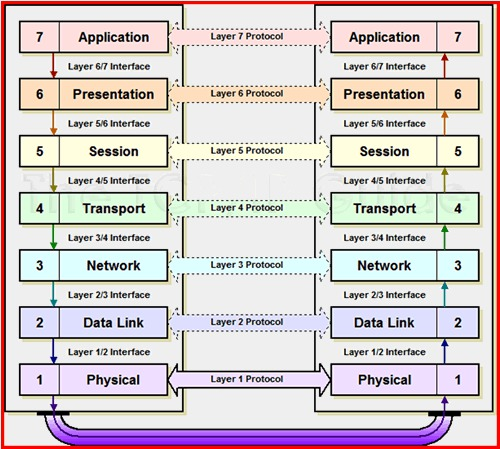
\includegraphics[width=12cm]{partie1/interaction1.jpg}
\end{figure}
\begin{figure}[H]
	\centering
	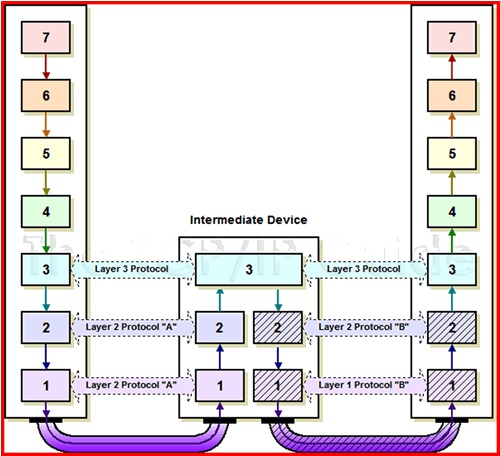
\includegraphics[width=12cm]{partie1/interaction2.jpg}
\end{figure}
\subsection{Transfert des données utilisateurs}
Les données des utilisateurs traversent toutes les couches du modèle OSI jusqu'au niveau physique qui génère le signal transmis sur le média. Chaque couche rajoute des informations de contrôle du protocole (PCI : Protocole Control Information) aux données qui lui sont passées par l'entité supérieure qui demande le service (SDU : Service Data Unit). C'est l'encapsulation des données. Cet ajout détériore les performances de débit mais sont nécessaires pour assurer les services des diféfrentes couches: adressage, contrôle d'erreurs, contrôle de flux\ldots

Cette structure est aussi appelée aussi ``structure en pelure d'oignon''.

Les données sont échangées entre les entités de même niveau qui savent les interpréter. C'est le protocole de communication qui définit le format des unités de données échangées (PDU: Protocol Data Unit) et les règles de communication.

\begin{figure}[H]
	\centering
	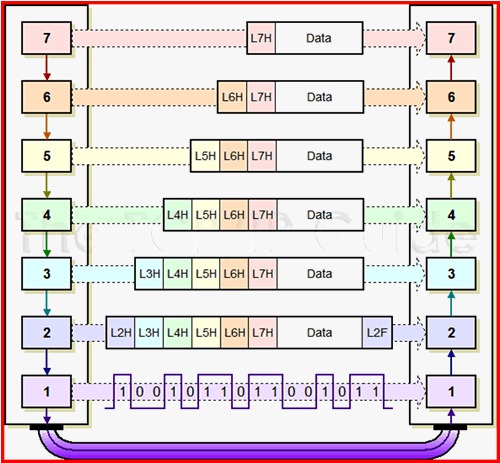
\includegraphics[width=15cm]{partie1/encapsulation.jpg}
\end{figure}

\paragraph{Segmentation/Réassemblage} Lorsque le service fourni par la couche $(N)$ fixe une limite de taille sur les données trop petites par rapport au service de la couche $(N+1)$, la couche $(N+1)$ découpe les $(N+1)-SDU$ en plusieurs fragments correspondant chacun à un $(N+1)-PDU$ avant envoi. À la réception, la couche $(N+1)$ concatène les fragments pour retrouver le $(N+1)-SDU$ initial.

\subsection{Intéractions entre entités}
Une couche donnée fournit un ensemble de services au niveau supérieur, les services sont invoqués par des primitives. Dans le Modèle OSI, les primitives sont désignées par un nom précédé de la première lettre du nom anglais de la couche. Par exemple, \texttt{$T\_$CONNECT} est une primitive de la couche Transport, \texttt{N$\_$DATA} une primitive de la couche Réseau.

Il y a 4 types de primitives de service :
\begin{itemize}
	\item Requête: une entité sollicite un service pour faire   une activité;
	\item Indication: Informe d’un évènement;
	\item Réponse: réponse à l’évènement;
	\item Confirmation: informe de la demande de service;
\end{itemize}

